% vim: tw=80 noai
\documentclass[normaltoc,capchap,capsec,times]{abnt}
\usepackage[utf8]{inputenc}
\usepackage[T1]{fontenc}
\usepackage[brazil]{babel}
\usepackage[alf]{abntcite}
\usepackage[ordem=alf]{tabela-simbolos}
\usepackage{url}
\usepackage{graphicx}
\usepackage{listings}
\usepackage{verbatim}
\usepackage{subfigure}
\usepackage{multicol}
\usepackage{framed}
\usepackage{multirow}
% O comando abaixo define o diretorio onde devem ser colocadas as imagens.
% Neste caso o diretorio é ./imagens/
\graphicspath{ {./imagens/} }
\def\lstlistingname{Listagem}

%%%%%%%%%%%%%%%%%%%%%%%%%%%%%%%%%%%%%%%%%%%%%%%%%%%%
% Dados da monografia
%%%%%%%%%%%%%%%%%%%%%%%%%%%%%%%%%%%%%%%%%%%%%%%%%%%%

\newcommand{\meunome}{José Lucas dos Santos Borges}
\newcommand{\meutitulo}{Construindo um mecanismo para predição de momentos oportunos para interrupção de motoristas utilizando contexto}
\newcommand{\meusubtitulo}{}
\newcommand{\meuano}{2016}
\newcommand{\meuorientador}{Orientador: \profa\ Vaninha Vieira dos Santos}
\newcommand{\meucoorientador}{Co-Orientador: Alberto Vianna Dias}

%%%%%%%%%%%%%%%%%%%%%%%%%%%%%%%%%%%%%%%%%%%%%%%%%%%%

%% O comando \obs aqui definido permite que o autor faca anotacoes na
%% monografia que aparecem no PDF gerado. Para ativar o comando, descomente
%% a primeira linha e comente a segunda.
%% Exemplo de uso: \obs{Preciso melhorar este parágrafo...}

%\newcommand{\obs}[1]{\underline{\textbf{OBSERVAÇÃO}}: \emph{#1}}
\newcommand{\obs}[1]{}

\def\ordfem{\mbox{\raise .35em \hbox{\underline{\scriptsize a}\ }}}
\def\ordmasc{\mbox{\raise .35em \hbox{\underline{\scriptsize o}\ }}}
\def\profa{Prof\ordfem.}

%%%%%%%%%%%%%%%%%%%%%%%%%%%%%%%%%%%%%%%%%%%%%%%%%%%%

\begin{document}

% Capa com Brasão

\begin{titlepage}
   \begin{center}
    	%logotipo
               
\includegraphics[scale=0.3]{brasao_ufba} \\
	%\vspace{0.7in}
              \centering{ 
	      \bf{
	      \LARGE{
		\uppercase{UNIVERSIDADE FEDERAL DA BAHIA} \\
 	      }
	      \Large {
                   	\uppercase{INSTITUTO DE MATEMÁTICA} \\
	      }
                   \large {
                       \uppercase{DEPARTAMENTO DE CIÊNCIA DA COMPUTAÇÃO} \\
                  }
              } }
   \end{center}
   \vfill
   \begin{center}
       \bf{
       \large{\uppercase{\meunome}  \\  }
       }
   \end{center}
   \vspace{0.2in}
   \begin{center}
       \bf{
      	 \LARGE{ \uppercase{\meutitulo} } \\
      	 \Large{ \uppercase{\meusubtitulo} }
         \obs{\\ \Large{Esta versão da monografia contém comentários do autor.
          Para removê-los, redefina o comando LaTeX \texttt{obs}.}}
       }
   \end{center}

   \vfill
   \hspace{\stretch{1}}
   \vfill
   \begin{center}
      \normalsize{
          Salvador \\
          \meuano
       }
   \end{center}

\end{titlepage}

%comando abaixo cria uma capa redundante, mas como a capa com brasão foi 
% feita 'manualmente', não faz sentido usar este comando:
%\capa



%\folhaderosto
% o comando acima foi comentado para não criar uma folha de
% rosto redundante, já que ela feita 'manualmente' abaixo

\begin{titlepage}
 \vfill
 \begin{center}
   {\large \uppercase{ \bf{ \meunome\ } } } \\[7cm]
   {\Huge \uppercase{ \bf{ \meutitulo\ } } }\\[1cm]
   \vfill
   \hspace{.45\textwidth} % posicionando a minipage
   \begin{minipage}{.5\textwidth}
     \begin{espacosimples}
       \bf{
	Anteprojeto da Monografia apresentada ao curso de graduação em Sistemas de Informação,
	Departamento de Ciência da Computação, Instituto de Matemática, Universidade Federal da
	Bahia, como requisito parcial para obtenção do grau de Bacharel em Sistemas de Informação. \\
       }
     \end{espacosimples}
     \begin{espacosimples}
       \meuorientador
     \end{espacosimples}
   \end{minipage}
   \vfill
   Salvador \\
   \meuano
 \end{center}
\end{titlepage}


%% As listas a seguir sao opcionais:
%\listadetabelas
\listadesiglas
%\listadesimbolos

\sumario

% O conteudo da monografia esta' nos seguintes arquivos:
\chapter{Introdução}
\label{introducao}

Dirigir um veículo pode ser considerado uma tarefa complexa, já que envolve diversas pequenas ações coordenadas e
que dependem tanto de fatores externos quanto internos. Um motorista deve saber adaptar-se a diferentes situações,
agir apropriadamente perante cada uma delas e tomar medidas rápidas em caso de emergência.

Neste contexto, a interrupção inoportuna é um perigo que pode ser fatal, pois demanda atenção do motorista em um momento
onde a distração pode levar a um acidente. Um fato que corrobora isto é o de que pessoas levam até 27\% mais tempo para
concluir uma tarefa quando são interrompidas e tendem a cometer o dobro de erros \cite{bailey2006need}. Exemplos de
interrupções que podem ocorrer para motoristas são barulhos repentinos, conversas com passageiros e notificações em
seu celular.

Outra informação que sustenta esta hipótese é a de que ao demandar a atenção dos motoristas durante a execução de
tarefas complexas sua distração também aumenta, pois a quantidade de informação que um motorista pode assimilar
depende da complexidade de sua tarefa no momento \cite{schneegass2013data}.

Um dos meios pelos quais os motoristas recebem interrupções são via notificações em dispositivos móveis.
Diariamente, pessoas que utilizam qualquer tipo de dispositivo móvel recebem dezenas de notificações
\cite{pielot2014situ}. Tais notificações demandam a atenção do usuário e podem acabar interrompendo uma tarefa que
está sendo executada no momento, dado que a atenção humana é um recurso finito \cite{simon1971designing}.

Interrupções de motoristas já são um problema a ser considerado. Nos Estados Unidos, 10\% dos acidentes com morte, em 2014, tiveram relação
com algum tipo de distração e 13\% deste tipo de distrações estão relacionadas com o uso de celulares e \textit{smartphones}
\cite{distracted2014}. Diante disto, prevenir este tipo de distração relacionada a dispositivos móveis torna-se uma necessidade.

A utilização de dispositivos móveis durante a direção de veículos, apesar de ser proibido no Brasil, é liberado em alguns
outros países, como Estados Unidos (em alguns estados como Flórida e Colorado \cite{cellphoneuse, distracteddriving} e Suécia \cite{swedendrive}.

Ao identificar padrões nos dados contextuais que indiquem momentos oportunos para interromper motoristas, é possível
construir uma solução que os notifique apropriadamente a depender do contexto que eles se encontram. Este trabalho propõe
o desenvolvimento de um módulo que detecte momentos oportunos e inoportunos para notificação de motoristas, utilizando
apenas sensores de smartphone. Este módulo será incorporado ao aplicativo Meu Possante, que serve como um auxiliar de mecânica automotiva.

O módulo supracitado será responsável por gerenciar o momento de entrega de certas notificações ao dispositivo. Ao incluí-lo no código,
o aplicativo terá a garantia de que suas notificações não estão sendo entregues em momentos indevidos e colocando em risco a vida dos
motoristas que usam smartphone.

Neste trabalho a seguinte metodologia foi utilizada: inicialmente investigamos momentos oportunos para interrupção de motoristas a partir
da leitura de artigos da área. Tendo em mente os momentos escolhidos para este trabalho (curvas e mudança de faixa), buscamos limiares na
literatura que nos permitam identificá-los utilizando apenas sensores de smartphone. Com estes dados em mãos, um módulo foi desenvolvido
em Android nativo e incorporado em um aplicativo experimental. Por fim, elaboramos um experimento para avaliar a solução proposta.

O experimento foi feito usando lorem ipsum dolor sit amet, consectetur adipisicing elit, sed do eiusmod tempor incididunt ut labore et dolore
magna aliqua. Ut enim ad minim veniam, quis nostrud exercitation ullamco laboris nisi ut aliquip ex ea commodo consequat. Duis aute irure dolor
in reprehenderit in voluptate velit esse cillum dolore eu fugiat nulla pariatur. Excepteur sint occaecat cupidatat non proident, sunt in
culpa qui officia deserunt mollit anim id est laborum.

O restante deste trabalho está estruturado da seguinte maneira: O Capítulo 1 Lorem ipsum dolor sit amet, consectetur adipisicing elit, sed do
eiusmod tempor incididunt ut labore et dolore magna aliqua. Ut enim ad minim veniam, quis nostrud exercitation ullamco laboris nisi ut aliquip
ex ea commodo consequat. Duis aute irure dolor in reprehenderit in voluptate velit esse cillum dolore eu fugiat nulla pariatur. Excepteur sint
occaecat cupidatat non proident, sunt in culpa qui officia deserunt mollit anim id est laborum.

\chapter{Motivação}
\label{motivacao}
Dirigir um veículo pode ser considerado uma tarefa complexa, já que envolve diversas pequenas ações coordenadas e
que dependem tanto de fatores externos quanto internos. Um motorista deve saber se adaptar a diferentes situações,
agir apropriadamente perante cada uma delas e tomar medidas rápidas em caso de emergência.

Neste contexto, a interrupção inoportuna é um perigo que pode ser fatal, pois demanda atenção do motorista em um momento
onde a distração pode levar a um acidente. Um fato que corrobora isto é o de que pessoas levam até 27\% mais tempo para
concluir uma tarefa quando são interrompidas e tendem a cometer o dobro de erros \cite{bailey2006need}. Exemplos de interrupções que podem
ocorrer para motoristas são barulhos repentinos, conversas com passageiros e notificações em seu celular.

Diariamente, pessoas que utilizam qualquer tipo de dispositivo móvel recebem dezenas de notificações \cite{pielot2014situ}. Tais notificações
demandam a atenção do usuário e podem acabar interrompendo uma tarefa que está sendo executada no momento, dado que a
atenção humana é um recurso finito \cite{simon1971designing}.

Interrupções de motoristas já são um grave problema. 10\% dos acidentes com morte nos Estados Unidos em 2014 tem relação
com algum tipo de distração e 13\% deste tipo de distrações estão relacionadas com o uso de celulares e smartphones \cite{distracted2014}.
Diante disto, prevenir este tipo de distração relacionada a dispositivos móveis torna-se uma necessidade.

A utilização de dispositivos móveis enquanto se está dirigindo, apesar de ser proibido no Brasil é liberado em alguns
outros países, como Estados Unidos (em alguns estados como Flórida e Colorado \cite{cellphoneuse} \cite{distracteddriving} e Suécia \cite{swedendrive}.

Identificando padrões nos dados contextuais que indiquem momentos oportunos para interromper motoristas, é possível
construir uma ferramenta que os notifique apropriadamente a depender do contexto que eles se encontram.

\sigla{GPS}{Sistema de Posicionamento Global}

\chapter{Fundamentação}
\label{fundamentacao}
Este capítulo aborda os principais fundamentos teóricos envolvidos na notificação oportuna de motoristas,
tema central deste trabalho. São apresentados conceitos sobre contexto, interrupção e notificação.
Ao final são apresentados alguns trabalhos correlatos.

\section{Contexto}
\label{contexto}
Em 1991, \cite{weiser1991computer} cunha o termo "Computação Ubíqua", que se refere ao caráter invisível da
integração de dispositivos computacionais diversos e da adaptação dos mesmos à necessidade do usuário no momento.
Um elemento bastante importante para a Computação Ubíqua é o estudo do contexto.

Contexto é definido por \cite{dey2001understanding} como "Qualquer informação que pode ser utilizada para
caracterizar a situação de entidades (ex: um usuário, lugar ou objeto) e que é considerada relevante para
a interação entre um usuário e uma aplicação, incluindo o próprio usuário e aplicação". Esta definição é
a mais utilizada na área e provavelmente a mais aceita. Alguns exemplos de elementos de contexto são
localização do usuário, ambiente, identidade do usuário e tempo \cite{ryan1999enhanced}.

Diversos sensores podem ser utilizados para determinar informações sobre o contexto do usuário. Alguns exemplos são
sensores de localização (GPS), sensores de luz e som, acelerômetro e giroscópio.

Informações de contexto são importantes para definir o estado atual do usuário e do ambiente onde ele está inserido,
mas somente isto é insuficiente. Para utilizar estas informações satisfatoriamente é ideal que se construa um sistema
adaptativo e que supra as necessidades do usuário em tempo real utilizando as informações de contexto. Resumindo,
um sistema sensível ao contexto.

Sistemas sensíveis ao contexto são capazes de adaptar suas operações ao contexto atual, sem intervenção
explícita do usuário e têm como objetivo aumentar sua usabilidade e efetividade levando em conta elementos
de contexto \cite{baldauf2007survey}. \cite{abowd1999towards} afirma que um sistema é sensível ao contexto
se ele utiliza contexto para prover informações relevantes e/ou serviços para usuários, sendo que a relevância
depende das tarefas do usuário.

\section{Interrupção}
\label{interrupcao}

Segundo \cite{ferreira2004novo}, interrupção é aquilo que faz parar uma ação ou um estado; o ato de cortar a continuidade de
algo. A interrupção durante a execução de uma tarefa pode ter vários efeitos adversos. \cite{lewin1927untersuchungen} diz
que pessoas lembram melhor dos detalhes de tarefas que não foram interrompidas. \cite{zijlstra1999temporal} conclui que
pessoas cometem mais erros em tarefas após uma interrupção. \cite{gillie1989makes} afirma que as pessoas executam tarefas
mais vagarosamente após uma interrupção, se comparado com a performance pré-interrupção.

A literatura indica que interrupções durante uma tarefa são bastante nocivas para a execução da mesma.

\subsection{Interrupção de Motoristas}
\label{interrupcao-motoristas}

(...)

Vários problemas na execução de uma tarefa após uma interrupção, como os citados na seção \ref{interrupcao}, afetam o
motorista durante a direção de um veículo:

\begin{itemize}
  \item Ao não lembrar de detalhes do que estava fazendo antes da interrupção, o motorista pode esquecer de informações
  apontadas pela sinalização de trânsito;
  \item Ao cometer erros após uma interrupção, o motorista põe em risco a si mesmo e a seus pares, podendo causar acidentes
  de trânsito;
  \item Ao reagir mais vagarosamente após uma interrupção, o motorista fica vulnerável a ameaças externas que exijam de sua
  capacidade reativa;
\end{itemize}

%A tabela 3.5 relaciona potenciais problemas que podem ser desencadeados pelas interrupções, citados na seção
%\ref{interrupcao}, com o contexto de motoristas.

\subsection{Notificações e seu caráter interruptivo}
\label{notificacao}

\cite{iqbal2010notifications} define notificação como um sinal visual, audível ou táctil, gerado por uma aplicação
ou serviço e que passa informação para um usuário que está fora de seu foco de atenção. Em dispositivos móveis,
notificações geralmente são enviadas instantaneamente no momento em que ocorre alguma atividade que pode ser relevante
para o usuário quando a aplicação não está aberta, ex: Um email novo, uma mensagem de texto que acaba de chegar ou um
novo comentário em suas redes sociais. Em alguns casos o usuário toma ações imediatas após a chegada da notificação,
enquanto em outros ela é simplesmente ignorada. Essas ações dependem da importância da notificação e do contexto do
usuário \cite{sahami2014large}.

\begin{figure}[h]
\centering
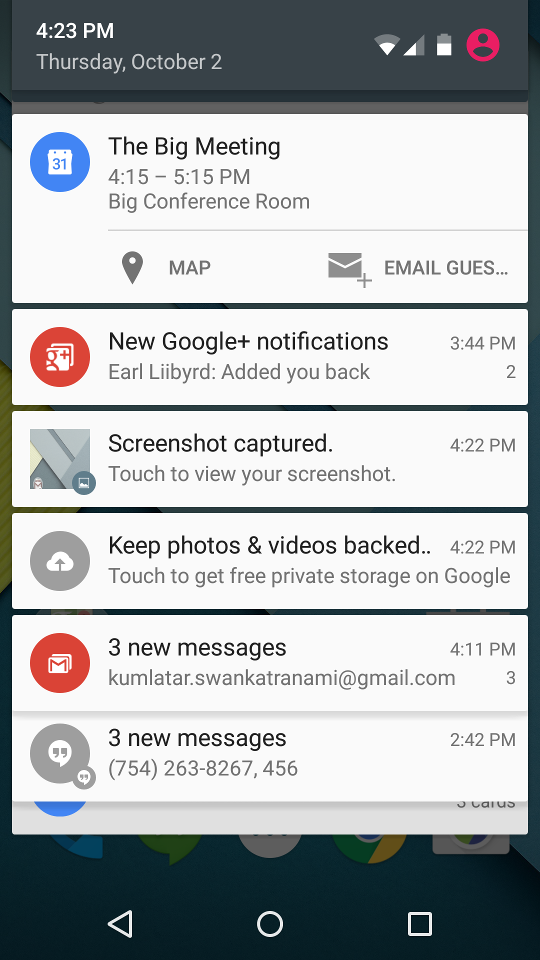
\includegraphics[width=0.3\textwidth]{notification_drawer}
\caption{Exemplo de notificações no Android \cite{notificationDrawer}}
\label{notification-drawer}
\end{figure}

Apesar da

\chapter{Proposta}
\label{proposta}
Este capítulo aborda os principais aspectos da proposta para o projeto final. As seguintes seções são apresentadas:
Metodologia, Resultados Esperados e Cronograma.

\section{Metodologia}
\label{metodologia}

\begin{enumerate}
  \item Serão identificados momentos oportunos para interrupção de motoristas a partir da leitura de artigos
relacionados;
  \item Serão escolhidos os sensores de smartphone que a aplicação utilizará para coletar dados contextuais, para
que seja possível identificar corretamente os momentos indicados no passo 1;
  \item Um aplicativo Android será criado para coleta de dados dos sensores escolhidos no passo 2;
  \item Será feita uma experimentação em situações reais de direção veicular, de forma a relacionar os valores indicados
nos sensores com momentos oportunos para interrupção;
  \item Será feita a investigação e escolha do melhor algoritmo de aprendizado de máquina para classificação dos dados,
baseado nos dados preliminares obtidos no passo anterior. Esta investigação será feita através da ferramenta Weka
\cite{hall2009weka};
  \item Será feito um estudo de caso para a avaliação dos resultados utilizando o modelo obtido no passo anterior;
\end{enumerate}

\section{Resultados Esperados}
\label{resultados}

Ao final deste trabalho espera-se ter um mecanismo que faça a predição automática de momentos oportunos para
interrupção de motoristas. No futuro, este mecanismo poderá ser implementado na forma de uma biblioteca, podendo assim
ser utilizada por qualquer aplicativo do sistema operacional Android.

\section{Cronograma}
\label{cronograma}

\begin{table}[h]
\centering
\resizebox{\textwidth}{!}{
\begin{tabular}{|r|c|c|c|c|c|c|c|c|c|}
\hline
\multicolumn{1}{|c|}{\multirow{2}{*}{Atividade}}                                                             & \multicolumn{2}{c|}{Dezembro} & \multicolumn{2}{c|}{Janeiro} & \multicolumn{2}{c|}{Fevereiro} & \multicolumn{2}{c|}{Março} & Abril     \\ \cline{2-10}
\multicolumn{1}{|c|}{}                                                                                       & 1ª quinz.     & 2ª quinz.     & 1ª quinz.     & 2ª quinz.    & 1ª quinz.      & 2ª quinz.     & 1ª quinz.    & 2ª quinz.   & 1ª quinz. \\ \hline
\begin{tabular}[c]{@{}r@{}}Pesquisa de momentos oportunos\\ para interrupção de motoristas\end{tabular}      & X             &               &               &              &                &               &              &             &           \\ \hline
\begin{tabular}[c]{@{}r@{}}Pesquisa de sensores utilizados para\\ obtenção de dados contextuais\end{tabular} & X             &               &               &              &                &               &              &             &           \\ \hline
\begin{tabular}[c]{@{}r@{}}Elaboração da arquitetura do\\ aplicativo\end{tabular}                            &               & X             & X             &              &                &               &              &             &           \\ \hline
\begin{tabular}[c]{@{}r@{}}Testes com sensores que serão\\ utilizados\end{tabular}                           &               &               &               & X            &                &               &              &             &           \\ \hline
Desenvolvimento do aplicativo                                                                                &               &               & X             & X            & X              & X             &              &             &           \\ \hline
Experimentação                                                                                               &               &               &               &              &                & X             &              &             &           \\ \hline
\begin{tabular}[c]{@{}r@{}}Escolha do algoritmo de\\ aprendizado de máquina\end{tabular}                     &               &               &               &              &                &               & X            &             &           \\ \hline
Estudo de caso                                                                                               &               &               &               &              &                &               & X            &             &           \\ \hline
Escrita da monografia                                                                                        &               & X             & X             & X            & X              & X             & X            & X           &           \\ \hline
Entrega do projeto                                                                                           &               &               &               &              &                &               &              & X           &           \\ \hline
Defesa do PF II                                                                                              &               &               &               &              &                &               &              &             & X         \\ \hline
\end{tabular}
}
\end{table}


\bibliography{monografia}

\end{document}
